\subsection{蒙特卡洛模拟数据假设}
网络上相关数据过少导致较难通过有监督的机器学习算法进行模型的训练,于是根据中国国内的真实数据进行数据建模,最后抽离出5个变量:
\begin{enumerate}
    \item 城市机场密度(将国内城市进行梯度划分)\cite{modood2018administrative};
    \item 机场停机位数量(将国内机场进行梯度划分)\cite{Pentadiine2019机场};
    \item 飞机时速(统计结果见附录~\ref{A:python-simulink}的\texttt{settings.py}文件);
    \item 飞机客容量(由搜索引擎搜索国内各大机场使用飞机型号及搭载乘客人数统计得出);
    \item 机场跑道容量\cite{wou2018跑道容量}。
\end{enumerate}

同时根据一定的规则(见附录~\ref{A:python-simulink}的\texttt{model\_airline.py}文),规划机场之间的航线,从而得到机场的客容量,由图~\ref{fig:path-a}与图~\ref{fig:path-b},从图像上来说两者基本符合。因此进一步模拟,产生各大机场的实时数据,我们选取第一梯队城市进行绘图,其中横坐标代表一天的秒数,纵坐标标示客流量,如图~\ref{fig:航空客流量},通过与能找到的少量真实数据进行比较,数据趋势大致相同,我们假设蒙特卡洛模拟可以模拟出机场总客流量。

\begin{figure}
    \centering
    \subcaptionbox{数据建模得出机场位置及航线图\label{fig:path-a}}%
        {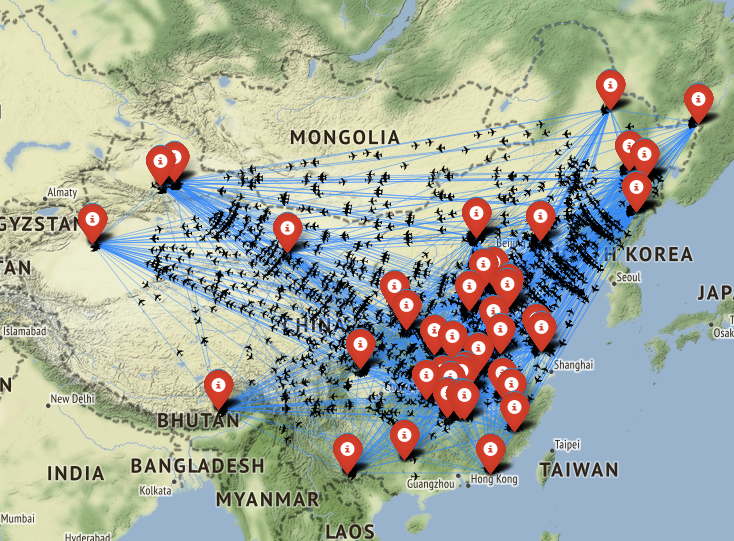
\includegraphics[width=.7\textwidth]{figures/path_python.png}} \\
    \subcaptionbox{飞常准世界航线图\label{fig:path-b}}%
        {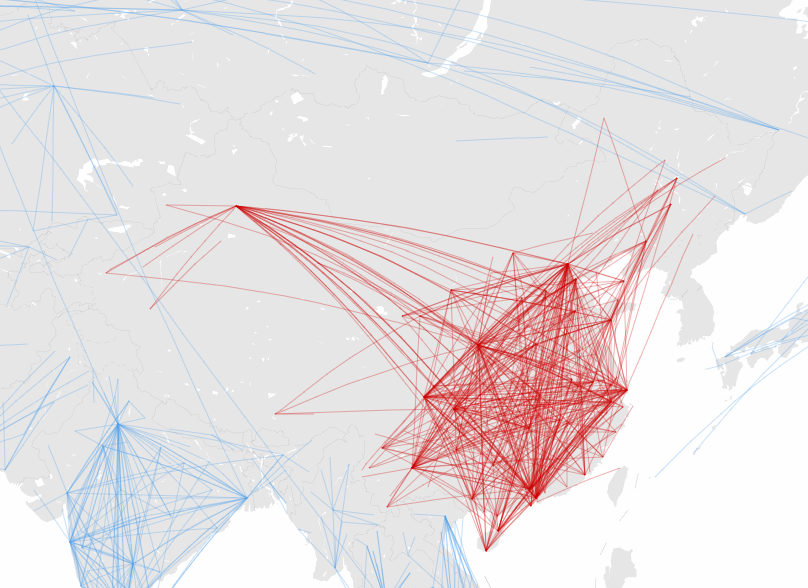
\includegraphics[width=.7\textwidth]{figures/path_variflight.png}}
    \caption{蒙特卡洛模拟与实际数据比较}\label{fig:path}
\end{figure}

\begin{figure}
    \centering
    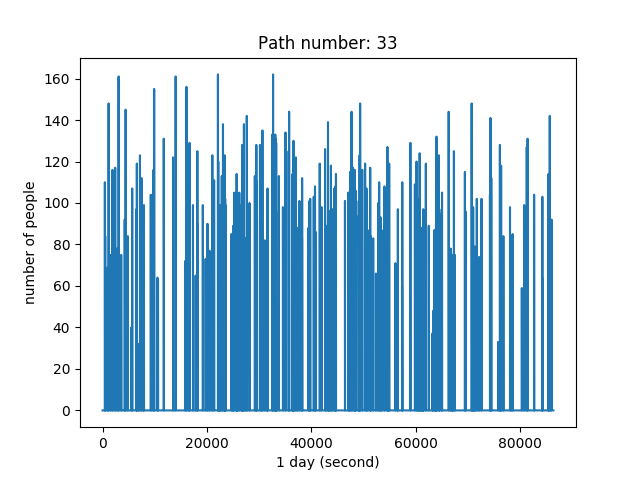
\includegraphics[width=.7\textwidth]{figures/航空客流量.png}
    \caption{实时模拟机场总客流量}\label{fig:航空客流量}
\end{figure}


\subsection{多元线性回归的五条基本假设}
\begin{enumerate}
    \item 问题一中预测司机载客概率$P$的模型可写为各解释变量的线性组合,即
        \begin{align*}
            P &= \beta_0 + \beta_1x_1 + \beta_2x_2 + \dots + \beta_kx_k + u \\
              &= \beta_0 + \sum_{i=1}^{k} \beta_ix_i + u.
        \end{align*}
        其中,$x_i (i=1,2,\ldots,k)$在本文中为各个解释变量,$k=6$,$\beta_i(i=1,2,\ldots,k)$在本文中为模型中各解释变量的系数,$u$为残差项;

    \item 假设模型含有$n$个观测值,则对于每一个观测值中的$k$个解释变量,均有且仅有一个对应的观测值;

    \item 假设各解释变量之间不相关,无完全共线性;

    \item 假设残差项关于所有解释变量的条件期望为0,即
        \[
            E(u|x_1,x_2,\ldots,x_k) = 0.
        \]

     \item 各解释变量满足同方差性,即
        \[
            Var(u|x_1,x_2,\dots,x_k) = \sigma^2,
        \]
        其中,$\sigma$是常数。
\end{enumerate}


\subsection{解释变量分布假设}
\begin{enumerate}
    \item 假设天气状态/航班延误状态服从两点分布,即
        \[
         Weather = 
         \begin{cases}
                1 & \text{航班延误/恶劣或极端天气} \\
                0 & \text{航班正常/天气晴好}
         \end{cases}
        \]
    
    \item 假设机场距乘客目的地距离$S_{out}$服从正态分布$N(10,3)$,单位为 \si{\kilo\metre}。
\end{enumerate}
